\documentclass[a4paper,man,natbib]{apa6}
\usepackage{microtype}
\usepackage{mathtools} % needed
\usepackage{hyperref}
\usepackage{tabularx}
\usepackage{lingex}
\usepackage[modulo,displaymath,pagewise]{lineno}

\newcolumntype{Y}{>{\raggedright\arraybackslash}X}
\usepackage[normalem]{ulem}
\hypersetup{hidelinks=True}
\newcommand*{\smex}[1]{\textit{#1}} % 'small example'
\newcommand*{\spex}[1]{``{#1}''} % 'spoken example'
\newcommand*{\term}[1]{\emph{#1}} % introducing a new term
\newcommand*{\citegen}[1]{\citeauthor{#1}'s~(\citeyear{#1})}
\newcommand*{\SE}{\mathit{SE}} % fix funny "SE" spacing
\newcommand{\resultsLog}[3]{$\beta = #1$, $\textnormal{SE} = #2$, $p #3$}
\newcommand{\resultsLM}[3]{$\beta = #1$, $\textnormal{SE} = #2$, $t #3$}

\usepackage[obeyFinal,textsize=tiny,backgroundcolor=yellow!60]{todonotes} % to get rid of all notes, pass
% `final' to the document class
\setlength{\marginparwidth}{2cm}


\title{Such gesture, very lie, wow}
\author{reorder(MC,JK,JL)}
\affiliation{Psychology, PPLS, University of Edinburgh}
\ifapamodeman{\note{\begin{flushleft}%
Josiah King\\
Philosophy, Psychology and Language Sciences\\
University of Edinburgh\\
7~George Square\\
Edinburgh EH8~9JZ, UK\\[1ex]
\url{J.P.J.King@sms.ed.ac.uk}
\end{flushleft}}}

\abstract{
Previous research suggests that, when questioning the veracity of an utterance, we perceive certain non-linguistic behaviours to indicate that a speaker is being deceptive.
Recently, work has highlighted how listeners' associations between speech disfluency and dishonesty happen at the earliest stages of reference comprehension, suggesting that the manner of spoken delivery influences pragmatic judgements concurrently with the processing of lexical information.
The studies presented here investigate the integration of visual information about a speaker into judgements of deception.
By studying the time-course of judgements of a speaker's (dis)honesty when presented with different visual cues to deception, we ask whether listeners are relying upon a rule-of-thumb association between visual cues and deception, or whether the link between gestures and perceived deception requires a more complex inferential process.
Participants saw and heard a video of a potentially dishonest speaker describe treasure being hidden behind a named object, while also viewing both the named object and a distractor object. 
Their task was to click on the object behind which they believed the treasure to actually be hidden.
Eye- and mouse-movements were recorded. 
Experiment 1 investigates the time-course of listeners' associations between visual cues and deception, using a variety of static and dynamic cues.
Experiment 2 focuses on a dishonesty-bias for adaptor (fidgetting) gestures, and asks whether listeners' judgements of deception correlate with how nervous they think the speaker appears in each video.
Results show that the visual modality can have a rapid and direct influence on pragmatic judgements, supporting the idea that communication is fundamentally multimodal.
Although the nonverbal delivery of an utterance is found to influence the early stages of reference comprehension, establishing deception-judgements based on visual cues appears to be more gradual than previous studies have suggested it is for spoken cues.
}


\begin{document}

%JK > mouse track discuss

\shorttitle{What do liars look like?}
\maketitle
\linenumbers
\noindent
%intro (%JK too long?)
That people deceive one another is an inescapable aspect of everyday communication.
After studying participants' social interactions over a one week period, \citet{DePaulo1996} concluded that people lie on average twice a day.
The idea that it is possible to detect deceit---that there are systematic differences in people's behaviour depending on whether they are telling the truth or a lying---has long captivated human interest in a variety of areas, from criminal interrogations to the business world.\footnote{Where, in some cases, ``how to lie'' is equally as important. See \url{https://www.marketplace.org/2008/02/18/busness/lying-essential-doing-business}.}
Much research has investigated the behaviours that listeners associate with lying, covering a wide range of multi-modal phenomena from speech disfluencies and vocal pitch to visual cues such as postural shifts and hand movements.
Few studies, however, have studied the time-course of inferences of deception, and fewer still have done so in a multi-modal setting.
The present experiments investigate listeners' associations of a speaker's nonverbal behaviour with the veracity of an utterance, studying how and when visual information about a speaker is integrated into pragmatic interpretations of speech.

%could actually start here?
In natural communication, speakers can convey information via multiple channels.
Along with spoken delivery, a speaker's gestures, postures and facial expressions all offer information which can have a bearing on the non-literal (or pragmatic) interpretation of a message, for instance conveying emotion \citep{Busso2004, Gregersen2005}.
One such pragmatic interpretation is the judgement of a statement's veracity.
Research suggests that there are many aspects of nonverbal delivery which we, as listeners, believe to be \term{cues-to-deception}. 
In an analysis of 33~studies, \citet{Zuckerman1981} found that nine out of the ten visual cues-to-deception that were investigated were believed to be indicative of deceit. 
In a further subset of 13~studies reporting relationships between cues and subsequent deception judgements (rather than explicit beliefs about cues), three (smiling, gaze, and postural shifts) of the four available visual cues were associated with perceived dishonesty.

Interestingly, listeners appear to make these associations independent of the reliability of cues as actual signals of deception: \citet{Zuckerman1981} found only two visual cues (shrugs and fidgetting) to be associated with actual deceit, and a  more recent meta-analysis found little evidence of a relationship between lying and almost any form of movement \citep{DePaulo2003}.\todo{see Jia comment in source}
%% Jia: another meta-analysis to cite here is Hartwig (2011) about cues to actual deception being weak (https://www.researchgate.net/profile/Maria_Hartwig/publication/51251661_Why_Do_Lie-Catchers_Fail_A_Lens_Model_Meta-Analysis_of_Human_Lie_Judgments/links/02bfe5109718134014000000/Why-Do-Lie-Catchers-Fail-A-Lens-Model-Meta-Analysis-of-Human-Lie-Judgments.pdf) - courtesy of the reviewer 2 who thinks my dialogue study is crap and implies that we should rely more on meta-analyses rather than individual studies...
Some studies have in fact found deception to be inversely related to the cues we think of as deceitful:
Lying has been linked with a \emph{decrease} in hand, arm, and leg movements \citep[e.g.][]{DePaulo1992, Ekman1989, Vrij1995}, as well as a reduction in illustrative gesturing \citep[e.g.][]{DePaulo2003, Cohen2010}.
Even speakers' post-hoc perceptions of their own gestures when lying have been found to be at odds with how they actually behave:
\citet{Vrij1996} found that after partaking in interviews in which they were in turn truthful and dishonest, \todo{try not to overuse em-dashes}participants believed that their movements increased when lying, even though a decrease actually occurred.
%(whether or not participants were informed before-hand that deception is usually associated with a decrease in movements had no effect).

%% MC: just said that in the previous paragraph!
% We tend to hold misguided judgements about which behaviours really co-occur with deception (see \citet{Vrij2000})
\todo{see source}Given that listeners' intuitions about deceitful behaviour are poor, the associations they make between visual information and deception are unlikely to have been learnt.
This is reinforced by the fact that in everyday communication, there are few occurrences where listeners are given immediate feedback on the honesty of a given utterance.
%
Why then do listeners hold such strong associations and beliefs between visual cues and lying?\todo{something went wrong with this sentence.  And are the beliefs `strong'?}
%
One suggestion is that these associations are based on a set of cues which listeners heuristically associate with deception \citep{DePaulo1982}.
% a rule-of-thumb based heuristic \citep{DePaulo1982}. (tautology!)
% not "the set of cues"
The heuristics may be predicated on lay beliefs about deception, or on introspection as a speaker rather than experience as a listener, but ultimately lead to the somewhat innaccurate model of what deceitful behaviour looks and sounds like. \todo{needs fleshed out a bit?}

\citet{Loy2017} investigated the association between lying and speech disfluency, and found support for the idea that listeners rely on a rule-of-thumb-based approach when judging the veracity of an utterance based on the way in which it is spoken.
\citeauthor{Loy2017} used a visual world eye- and mousetracking paradigm in which participants were presented with images of two objects, and heard utterances describing the location of some treasure purportedly hidden behind one of the objects.
These utterances were presented as having been elicited in a previous experiment, in which the speaker was said to have been lying some of the time.
Crucially, \citet{Loy2017} manipulated the manner of spoken delivery, with half of the experimental items containing a speech disfluency.
Participants were tasked with clicking on the object they \textit{believed} to be concealing the treasure, choosing either the object named in the utterance (indicating a judgement of honesty), or a distractor (indicating dishonesty).
They were more likely to judge disfluent utterances as dishonest than fluent ones (as indicated by a greater probability of clicking on the distractor in a disfluent trial). 
Importantly, disfluency resulted in an early bias in both eye and mouse movements towards the not-referred-to object.
This suggests that speech disfluency is already incorporated into listeners' ideas concerning deceptive speech, and has an immediate effect on their interpretation of an utterance. 

%%%%%%%%----HERE

Little is known, however, about whether such rapid integration of cues to deception might extend to the visual channel of communication. 
Adhering to a rule-of-thumb association may be feasible for spoken cues, and evidence suggests that some effects of speech interruptions on comprehension do not discern between a spoken \spex{um} and an artificial tone \citep{Corley2011}.
Co-speech movements, however, are substantially more varied than speech interruptions, serving as both potential markers of metacognitive states and planning processes, and as an alternative modality in which a speaker can convey semantic information (such as via an illustrator).
Any rule-of-thumb heuristic between visual information and deception must be refined enough to discern between the type/content of co-speech movements, or risk potentially over-attributing any cue as a sign of deceit.
Furthermore, listeners also associate static visual cues with deception \citep[e.g. eye-gaze,][]{Zuckerman1981a}, suggesting that judgements of dishonesty are not linked just to variations in movement, but to a wide array of visual cues. 
It is not clear how such a heuristic might map such varied visual information to deceit.

An alternative account to the rule-of-thumb explanation suggests that non-linguistic information might influence listeners' judgements of deception via a form of on-the-go speaker-modelling: 
When presented with a possibly deceitful utterance, listeners might be inferring information about a speaker's metacognitive states, linking visual and spoken cues to deception via the perception of, e.g. nervousness, or cognitive effort. 
Such an account requires more complex inferential processing, being a two-step inferential process linking gesture to, e.g. anxiety, which is in turn attributed to the intention to deceive.
%% Jia: also I'm not sure whether it's best to call it a form of speaker-modelling here or not - it is speaker modelling but it doesn't seem to quite contrast with the rule-of-thumb account (wouldn't introspection as a speaker, which you mention earlier, create some sort of a speaker model as well?). I might be overthinking things, but it's worth thinking about whether this could be called something more specific (or see if Martin cares...)
%JK link car-horns paper in here?

Research is needed to distinguish between a speaker-modelling account and a rule-of-thumb heuristic account of the processes underlying how people interpret visual cues as indicative of deception.
This has wider implications on how listeners integrate visual information to inform comprehension of the pragmatic content of communication.
To date, the link between visual cues and perceived deceit has been studied only in terms of after-the-fact judgements, or assessing listeners' explicit beliefs about cue validity (see \citealt{Vrij1996a, Zuckerman1981a}).
Studying the time-course of judgements about the honesty of an utterance which is accompanied by different visual cues can help to shed light on how these cues are integrated.


We extend the `treasure game' paradigm from \citet{Loy2017} to include a video of the potentially deceptive speaker describing the location (behind one of two objects) of some hidden treasure on the screen while listeners attempt to guess the true location based on whether they believe the speaker to be lying or telling the truth. 
%%% Jia: we should include a figure of the display here %%%
Crucially, we manipulate the presence or absence of potential visual cues to deception in the video.
Experiment 1 investigates how the time-course of deception-judgements varies between different types of cues, including both increases in movement and different static postures.
If listeners associate visual cues with deception via a rule-of-thumb association, then a bias towards the not-referred-to object should occur early in trials presenting visual cues to deception.
In Experiment 2 we explore the possible role of perceived anxiety as an intermediary step in judgements about a speaker's honesty.
Concentrating on adaptor gestures (fidgeting movements), having been previously linked with anxiety \citep{Gregersen2005}, we ask whether listeners' judgements of deception are driven by their perceptions of how nervous they think the speaker to be when producing these gestures.

\section{Experiment 1}
Experiment 1 makes use of eye- and mouse-tracking to investigate the time course of listeners' judgements about the honesty of an utterance, and how these judgements are influenced by the occurrence of various visual cues. 
The experiment was presented as a `lie detection game', with each trial presenting a video and audio recording of a potentially deceptive speaker describing the location of some hidden treasure on the screen (behind one of two possible objects). 
Participants were tasked with clicking on where they believe the treasure to be hidden based on their judgement of the speaker's honesty.
We employed 3 types of visual cues --- trunk movements, adaptor gestures, and different postures --- investigating if and how listeners associated any of these with deception.
%% (add) Our results show that...


\subsection{Materials}
Visual stimuli consisted of the same 120 line drawings from \citet{Snodgrass1980} which were used in \citet{Loy2017}, sixty of which served as referents and the other sixty distractors.
Referents were randomly paired with distractors and presented in across sixty trials. 
In each trial, the speaker named one object (referent) as that which concealed the treasure; the other object is hereafter named the distractor.
Each referent was associated with a recording specifying the image as the object that the treasure was hidden behind (``The treasure is behind the <referent>'').
Along with these images, each trial presented a video (with no audio) of a person who was purported to be the speaker of the utterances. 
So that videos could be counterbalanced across referents, and thus across utterances, the face of the person in the video was blurred. 
This meant that, when presented with a given utterance, it was believable that both audio and visual stimuli had been produced concurrently. 

Sixty videos (30 Cue, 30 No-Cue) were created. 
The thirty no-cue videos were comprised of ten recordings (each presented thrice) of a speaker sitting motionless with her hands on either side of a tablet on a table, upon which the referent, distractor, and location of treasure was purported to be displayed.
Ten videos presented the speaker making one of five trunk movements, ten presented various adaptor gestures (e.g. finger tapping, head tilts), and ten presented the speaker sitting motionless but in a different posture to that of the no-cue videos (e.g. hand on chin, arms crossed, etc).

%JK essentially, we've got utterance initial (trunk movmements); utterance medial (adaptor gestures) and utterance global (posture)
A variable video-to-speech-onset was adopted for the 30 cue videos, controlling the position of the cues relative to speech. 
%%Jia: sorry, I can't fully remember what we did at this point - I thought it was gesture-to-speech onset (rather than video to speech)? 
%JK it was video-to-speech - basically we tried to audio and video to seem believable. i don't think we measured when exactly the cues began/stopped other than the trunk movements.
For trunk movements, the frame at which the movement ended was identified and used as the point of utterance onset (Mean onset = 1430ms, SD = 440ms).
To control for any sensitivity to the duration of pre-utterance video (which could be interpreted as speech-initiation time, in turn a potential cue to deception), these durations were matched in the no-cue videos.
For adaptor gestures, the movements overlapped with speech, with the duration of overlap determined individually for each video according to what looked most believable to the researchers (Mean = 1370ms, SD = 410ms). 
%JK is this speech gesture overlap, or gesture_onset? or speech onset? check and rewrite
These durations were matched in the videos that presented the speaker sitting in a different posture.

As with \citet{Loy2017}, 20 critical referents were counterbalanced across two lists. 
Each list contained 10 cue and 10 no-cue videos.
The 10 cue videos were trunk movements since we predicted these to be the most likely visual cue to elicit judgements of deception\citep{Vrij1996a}
%Jia: think we should try and provide a cite for this (one of the Vrij studies?)
% JK: have done, but it's not great. Vrij splits "trunk movements" (moderate assocation) and "postural shifts" (strong association). I think we used trunk movements to mean postural movements. It's not clear what Vrij uses. 
%% Jia: hm fair enough, I thought it would be relatively straightforward to find a useful cite, but I guess Vrij can be quite unclear. Let's leave it for now and I'll see if I come across a more useful one at all
The remaining 40 referents were randomly paired with one of the remaining videos (10 adaptors, 10 different postures, 20 no-cue) for each participant, with no repetition of referents across videos.

\subsection{Procedure}
Stimuli were displayed on a 21~in.\@ CRT monitor, placed 850~mm from an Eyelink~1000 Tower-mounted eye-tracker which tracked eye movements at 500~Hz (right eye only). 
Audio was presented in stereo from speakers on either side of the monitor. 
Mouse coordinates were sampled at the frame rate of the videos (25~fps, or every 40~ms).
The experiment was presented using OpenSesame version~3.1 \citep{Mathot2012}.
Eye movements, mouse coordinates and object clicked (referent or distractor) were recorded for each trial.

Figure \ref{fig:v1_trial} presents a sample trial from the experiment. 
\begin{figure}[Ht]
  \centering
	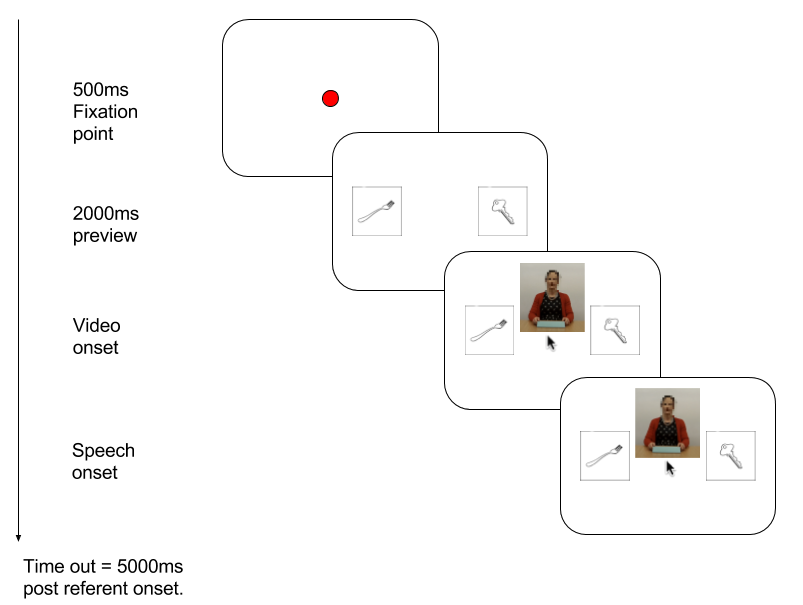
\includegraphics[width=\linewidth]{./img/e7_trial.png}
  \caption{Procedure of a given trial, Experiment 1}
  \label{fig:v1_trial}
\end{figure}
Between trials, participants underwent a manual drift correct to ensure accurate recordings from the eye-tracker.
After this the fixation dot turned red for 500ms. 
This was replaced by the two objects (referent and distractor), which were displayed on the screen for 2000ms.
The video then appeared and the cursor was centred and made visible.
Playback of the utterance began after the variable speech onset associated with each video (Mean = 1410ms, SD = 410 ms). 

The instructions emphasised that the videos participants saw were recorded from a previous experiment, in which the speaker had to describe the location of some hidden treasure with the aim of misleading the listener into choosing the wrong location.
Participants were instructed to click on the object behind which \textit{they believed} the treasure to be hidden, with the overall aim of accumulating as much treasure as they could across the experiment.
Participants received no feedback after their object clicks, except on bonus trials, which are described in the next section.

Participants completed five practice trials (one of which was presented as a bonus round) prior to the main experiment. 
Two of these included no cue, two displayed the speaker in different postures, and one displayed the speaker making a trunk movement.

\subsection{Bonus Rounds}
To maintain motivation throughout the study, participants were told that there were a number of ``hidden bonus rounds'' which offered more treasure than regular rounds.
25\% of trials (half in the cue condition; half in the no-cue condition) were randomly designated as bonus rounds for each participant.
These trials were visually identical to regular trials, with the exception of a message informing participants that they had successfully located bonus treasure following their mouse click (regardless of the object chosen).

Participants were also told that the top scorers would be able to enter their names on a high-score table, which was shown at the beginning of the experiment. 

\subsection{Post-test Questionnaire}
Participants were asked to complete a short post-test questionnaire. 
The questionnaire contained three questions, the most important of which asked if participants noticed anything odd about the visual or audio stimuli.
Any participant who indicated that they noticed anything unusual was then verbally questioned, to decide whether they believed that the speech and gesture had been produced naturally and simultaneously.
All participants were subsequently debriefed, during which they were told that the audio and video were created separately and stitched together, and asked again verbally if they noticed anything unusual in that respect. 
Their responses to the questionnaire and debrief were used as exclusion criteria for the analysis.

\section{Results}
Twenty-four native English speaking participants took part in the experiment for a planned sample size of twenty.
Participants were recruited from the University of Edinburgh community, and participated in return for a payment of \pounds{}4.
Data from four participants who indicated suspicion of the proposed origins of the audiovisual stimuli based on the post-test questionnaire and/or debrief were removed from all analyses.

\subsection{Analysis}
Analysis was carried out in R version~3.4.4 \citep{Rbase2017}, using the lme4 package \citep{Bates2015}. 
Trials in which participants did not click on either the referent or distractor (0.003\% of trials) were excluded from all analyses. 

Object clicked (referent or distractor) was modeled using mixed effects logistic regression, with fixed effects of cue type (No-Cue, Different Postures, Trunk Movements, Adaptor Gestures) and video-to-speech duration (Z-scored), thus controlling for any possible effect of perceived speech latency on judgements of dishonesty.
Cue type was dummy coded with No-Cue as the reference level.
Random intercepts and slopes for cue type and video-to-speech were included by-participant, along with random intercepts by-referent.
Reaction times (measured from referent onset) were modelled with the same fixed and random effect structure.
Following \citet{Lo2015}, we compared mixed effects logistic regression models which specified an identity link function, assuming gaussian, gamma and inverse gaussian distributions.

In previous studies using the treasure game paradigm, eye- and mouse- movements have been analysed over the time window starting at the onset of the referent name and extending for 800~ms; just beyond the duration of the longest referent in the analysis (776~ms). 
The current study included a larger set of referents, the longest of which was 1062~ms, so this window was extended to 1100~ms.

Eye fixation data was averaged into 20~ms bins (of 10 samples) prior to analysis.
For each bin, we calculated the proportions of time spent fixating the referent or the distractor, resulting in a measure of the proportions of fixations on either object over time.

The position of the mouse was sampled every 40~ms.
Using the $X$ coordinates only, we calculated the number of screen pixels moved and the direction of movement (towards either referent or distractor).
We then calculated the cumulative distance travelled towards each object over time as a proportion of the cumulative distance travelled in both directions up until that time bin.
Movements beyond the outer edge of either object were considered to be `overshooting' and were not included in calculations (0.8\% of samples).
Eye- and mouse- biases were calculated from the proportions of referent to distractor fixations, and were subsequently empirical logit transformed \citep{Barr2008}. 
In these measures, a value of zero indicates no bias towards either object, and positive and negative values indicate a bias towards the referent and distractor respectively.

Eye and mouse data was modelled over the time window from 0 to 1100~ms post-referent onset using linear mixed effects models, with fixed effects of time, cue type, and their interaction.
Random intercepts and slopes for time were included both by-referent and by-participant, along with by-participant random effects of cue type.
Following \citet{Baayen2008}, we considered effects in these models to be significant where $|t|>2$.

%JK Maybe just get rid of this analysis? >>
%As visual inspection of the time-course of fixations towards either object suggested that there was a later effect of visual cues in participants' decision of which object to click on, growth curve analysis (see \citealt{Mirman2008}) on the empirical logit transformed referent-to-distractor bias was used to investigate this further. 
%This analysis was conducted over the time window from 0 to 1815~ms post-referent onset (average time-to-click), and included 3 degrees of orthogonal polynomials for time, based on the pattern of the elogit referent-distractor bias having 2 turning points. 
%These time polynomials, along with their interaction with cue type, were included as fixed effects in a linear mixed effects model, with random intercepts and slopes for all time polynomials both by-participant and by-referent.


\subsection{Object clicks} 
Across the experiment, participants clicked on the referent in 55\% of trials and the distractor in only 45\%.
Table \ref{table:v1_clicks} shows the percentage of clicks across all participants to either object following different types of visual cue.
When presented with an utterance accompanied by no-cue, participants showed a bias toward a final interpretation of the utterance as truthful, with more clicks to the referent than the distractor \resultsLog{0.62}{0.16}{<0.001}.
Analysis showed that all visual cues resulted in a reduction of this bias, with adaptor gestures (\resultsLog{-1.03}{0.34}{=0.003}) showing a greater change than different postures and trunk movements (\resultsLog{-0.72}{0.31}{=0.017} and \resultsLog{-0.62}{0.26}{=0.018} respectively). 
The duration of video shown prior to the beginning of speech was not found to be associated with which object was eventually clicked.
%Comparisons --- via both AIC and BIC --- of reaction time models suggested that an inverse gaussian distribution provided the best fit to the observed data. 
Neither cue type nor duration of video prior to speech was associated with a significant change in reaction times.

\begin{table}
\caption{Breakdown of mouse clicks recorded on each object (referent or distractor) by type of visual cue for Experiment 1}
\label{table:v1_clicks}
\begin{tabularx}{\linewidth}{YYYYY}
\hline
& No-Cue & Different Posture & Trunk Movement & Adaptor Gesture \\
Clicks to Referent & 63.8\% & 48.0\% & 49.7\% & 41.5\%  \\ 
Clicks to Distractor & 36.2\% & 52.0\% & 50.3\% & 58.5\% \\
\hline
\end{tabularx}
\end{table}

\subsection{Eye movements}
Figure \ref{fig:v1_eye} shows the time-course of fixations to referents and distractors over 2000~ms from referent onset, split by each type of video.

Analyses conducted over the period from referent onset to 1100~ms post-onset (duration of the longest referent) showed that, when presented with a no-cue video, participants displayed a fixation bias towards the referent which increased over time (\resultsLM{1.15}{0.29}{=3.99}).
For videos which presented the speaker either in a different posture, or producing an adaptor gesture, this increasing bias to the referent was significantly reduced
(\resultsLM{-0.97}{0.13}{=-7.37}, \resultsLM{-0.59}{0.13}{=-4.50}), but this was not the case for videos of trunk movements (\resultsLM{-0.25}{0.15}{=-1.67}). 


%Growth curve results
%Figure \ref{fig:v1_gca} shows the time-course of the elogit referent-distractor bias, alongside the fitted values from the growth curve model. 
%Growth curve analysis over the period from referent onset to 1815~ms post-onset (mean click time) showed that when presented with a no-cue video, participants showed a tendency to fixate on the referent over the course of this time period (\resultsLM{0.67}{0.11}{=6.03}). 
%Significant effects of cue type on the intercept term indicated lower overall referent fixations during this period after viewing a different posture (\resultsLM{-0.36}{0.04}{=-10.10}), a trunk movement (\resultsLM{-0.29}{0.4}{=-7.36}), or an adaptor gesture (\resultsLM{-0.67}{0.4}{=-18.89}), in comparison to the no-cue videos.
%Significant interactions of cue type and the linear time coefficient indicate that this reduction in referent-bias dependent on cue type increases over the course of the window, with adaptor gestures showing a larger reduction relative to no-cue videos (\resultsLM{-116.89}{11.62}{=-10.06}) than different postures (\resultsLM{-75.41}{11.65}{=-6.47}) and trunk movements (\resultsLM{-58.78}{12.97}{=-4.53}). 
% JK: Beyond this, different posture videos showed a more gradual initial tendency towards the referent relative to the no gesture videos (\resultsLM{39.83}{11.64}{>2}) and trunk movement videos showed an increased ?? -- the little curve at the end.. (\resultsLM{33.50}{12.75}{>2}).


\begin{figure}[Ht]
  \centering
	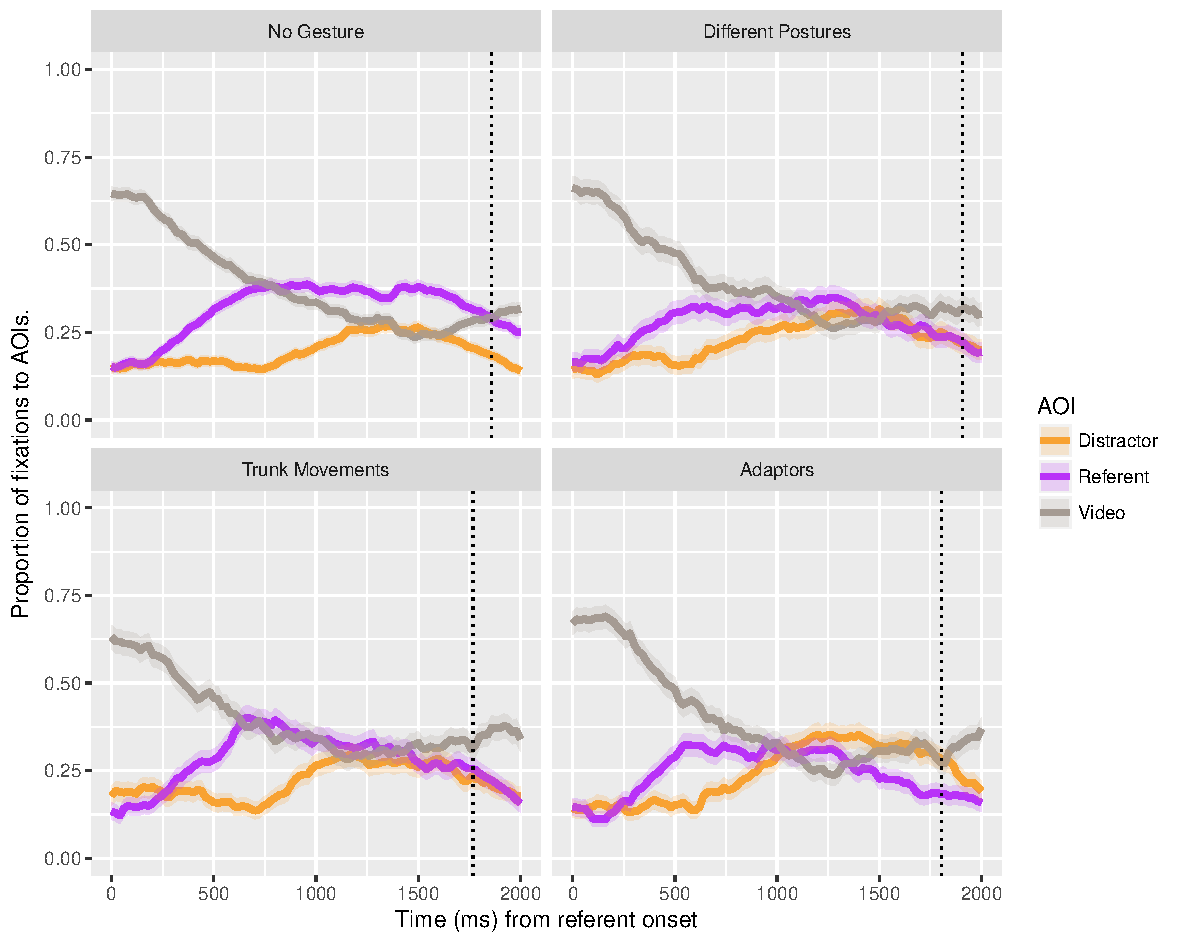
\includegraphics[width=\linewidth]{./img/e7_fixations.pdf}
  \caption{Eye-tracking results for Experiment 1: Proportion of fixations to each object (referent or distractor) and the video, from 0 to 2000 ms post-referent onset, calculated out of the total sum of fixations for each 20~ms time bin. Shaded areas represent $\pm$ 1 standard error of the mean.}
  \label{fig:v1_eye}
\end{figure}

\begin{figure}[Ht]
  \centering
	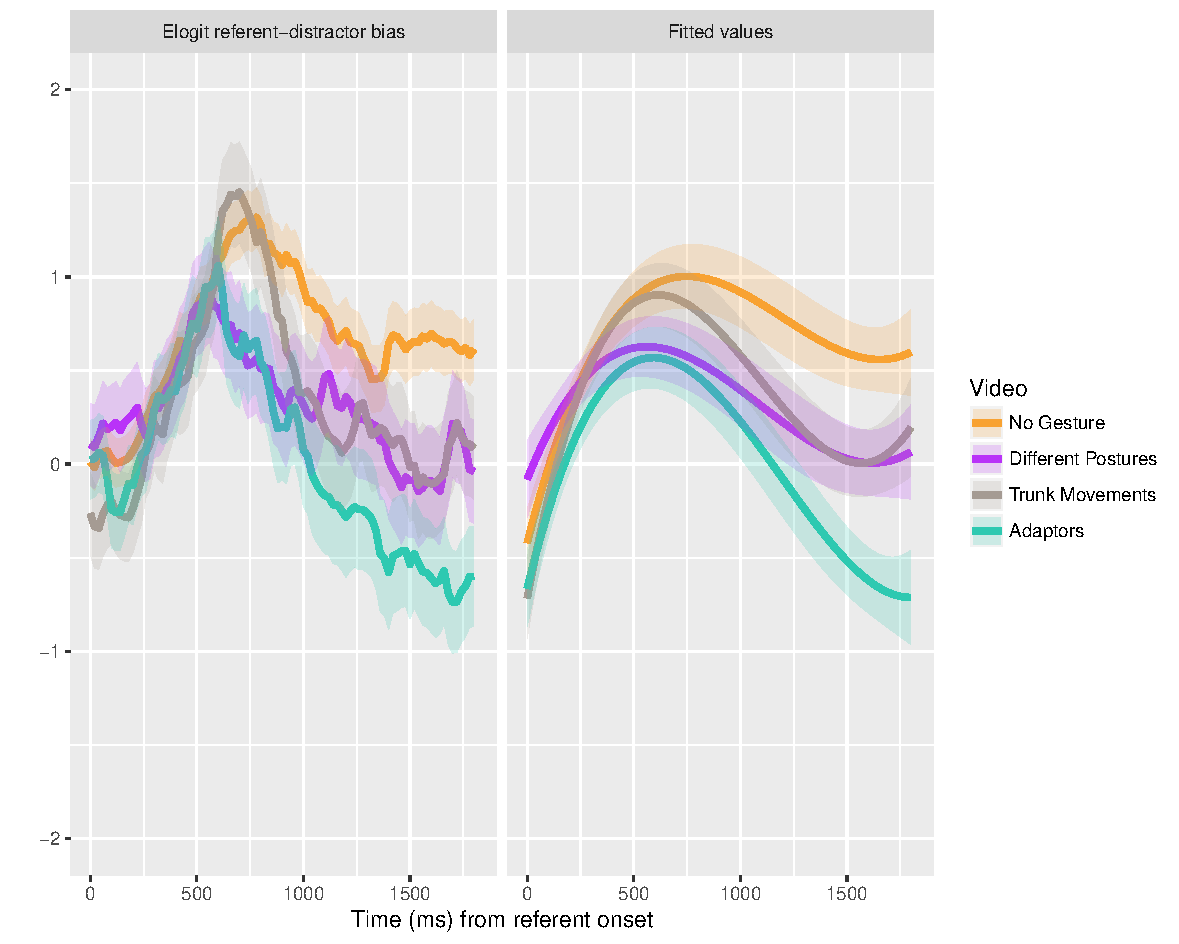
\includegraphics[width=\linewidth]{./img/e7_gcamodel.pdf}
  \caption{Elogit referent-distractor bias, and fitted values from growth curve analysis}
  \label{fig:v1_gca}
\end{figure}


\subsection{Mouse movements}
Figure \ref{fig:v1_mouse} shows the time-course of the proportions of cumulative distance the mouse moved towards the referent and distractor for 2000~ms from referent onset, split by each type of video.
Analysis on the time window from 0 to 1100~ms post-referent onset patterned with the eye-tracking data:
When viewing a speaker making no visual cue, participants showed an increasing tendency to move towards the referent over this period (\resultsLM{1.08}{0.22}{=4.86}).
As with the eye-movements, different postures and adaptor gestures resulted in a weakening of this referent-bias (\resultsLM{-0.81}{0.13}{=-6.28} and \resultsLM{-0.77}{0.13}{=-5.87} respectively), but trunk movements did not (\resultsLM{-0.10}{0.14}{=-0.69}). 

\begin{figure}[Ht]
  \centering
	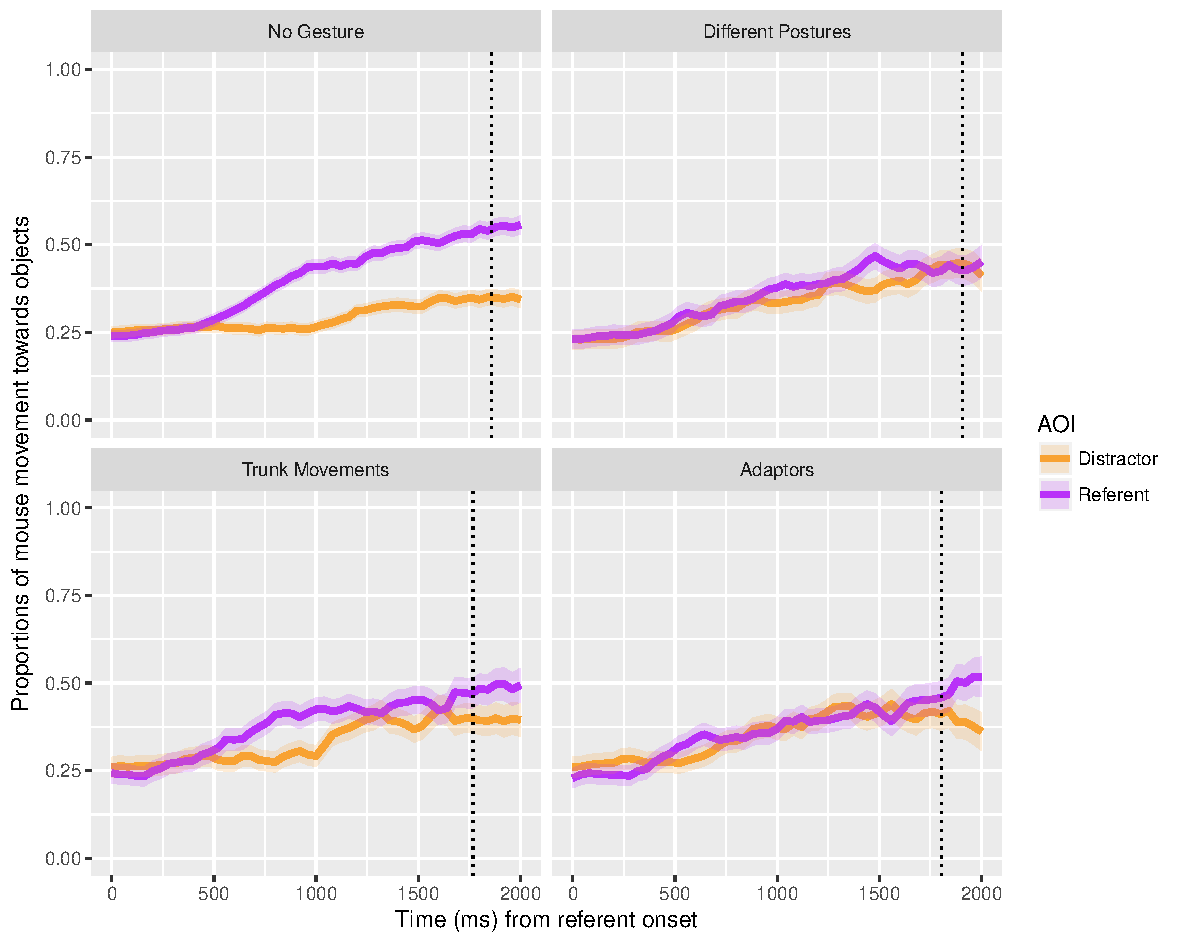
\includegraphics[width=\linewidth]{./img/e7_mouset.pdf}
  \caption{Mouse-tracking results for Experiment 2: Proportion of cumulative distance traveled toward each object from 0 to 2000 ms post-referent onset. Proportions were calculated from the total cumulative distance participants moved the mouse until that time bin (from video onset, when cursor was made visible). Shaded areas represent $\pm$ 1 standard error of the mean.}
  \label{fig:v1_mouse}
\end{figure}


\section{Discussion}
Experiment 1 investigated how the pragmatic inferences listeners make about a speaker's honesty are influenced by the presence of different types of movements and postures. 
We measured eye- and mouse- movements of participants who were presented with a task in which they made decisions about the true location of some treasure based on audio and video of a potentially deceptive speaker making a statement about the treasure's location.
Participants were thus making implicit decisions about the honesty of each utterance.
Our findings suggest that a speaker's nonverbal behaviour influences listeners' judgements about (dis)honesty.

As in previous studies using versions of this paradigm \citep{Loy2017, King2018}, participants showed a tendency to interpret an utterance as truthful when it had been presented without any potential cue to deceit.
Utterances presented alongside any cue --- both movement and different postures --- weakened this tendency, supporting previous findings in the deception literature that listeners' final judgements of deception are influenced by a speaker's nonverbal behaviour.
However, only the presence of adaptor gesturing resulted in significantly more final judgements of deception than truthfulness (as indicated by more clicks to the distractor over the referent).

The influence of the visual channel was also evident in participants' early stages of utterance processing. 
Across videos both with and without a cue, participants showed an initial tendency to fixate and move the mouse toward the referent over the distractor; however, videos of different postures and adaptor gestures weakened this referent bias.
Interestingly, this was not the case for videos of the speaker producing a trunk movement, despite the movement having been presented at an earlier point---relative to speech---than the adaptor gestures.
One possible explanation for this could be due to the fact that at the point of referent onset, the audiovisual information immediately available to the listener was comparable to the no-cue videos, since the trunk movements would have ended by that point.

This explanation, however, is at odds with the bias towards judgements of deception following utterance-initial disfluencies observed in previous work \citetext{\citet{Loy2017}, Experiment 1}.
We cannot at present reconcile this discrepancy, although we suggest that they may point toward differences in the mechanisms underlying the integration of audio and visual cues with a pragmatic inference.
Future research could explore the simultaneous integration of audio and visual information during judgements of deception, comparing the relative time course with which the two are integrated by the comprehension system.

Despite this evidence of an early effect of visual cues on reference comprehension, the point at which listeners' preferences toward the referent tended to be matched (or overtaken, in the case of adaptor gestures) by a preference for the distractor appeared at approximately 1000~ms post-referent onset. 
In other words, the distractor-bias following visual cues to deception appeared relatively late in processing.
This contasts with previous studies using audio-only versions of the `treasure-game' paradigm: Participants in \citet{Loy2017} showed little to no initial referent-bias following a disfluent utterance, with a distractor-bias appearing approximately 600~ms post-referent onset following both utterance-initial and utterance-medial disfluencies. 
This difference could be a result of visual information in the videos detracting participants from fixating the two objects. 
In particular, the integration of visual information into a judgement of deception could be delayed relative to that with a judgement of truthfulness: 
This would explain why listeners' distractor-bias in the cue conditions was delayed, despite the fact that their initial referent-bias across all conditions emerged early on at approximately 300~ms post-referent onset --- a point comparable to previous studies (\citealt{Loy2017, King2018}). 

Judgements of deception took substantially longer to unfold than in previous studies using the same paradigm (minus the video component), suggesting that listeners might be drawing links between visual cues and dishonesty via a more cognitively demanding process than a straightforward heuristic.
Although visual information was found to influence the early stages of comprehension, it is unclear whether this should be taken as evidence of emerging judgements of deception, or merely as differences in visual saliency between experimental stimuli (e.g., a trunk movement vs. an adaptor).

To investigate further the possibility that the association between visual cues and deception passes via some sort of modelling of the speaker's cognitive state, we conducted Experiment 2, focussing on perceived nervousness in the speaker.
Whilst lying can at times be a means of avoiding negative emotions (i.e. avoiding guilt, shame or embarassment by lying about one's transgressions), the act of producing any lie can be a potential catalyst for emotional response.
One such response, which fits well in the context of our experiment (the treasure-hunt game), is the fear of being detected.
Leakage of cues to deception has been attributed to fear of detection \citep{Ekman2009}, and this fear may be either related to the behaviour they are hiding with the lie, or the implications of being found to be dishonest \citep{Schlenker2001}. 
There is also a characteristic body-language which is associated with anxiety \citep[see also][]{Gregersen2005}. 
Experiment 2 explores the possibility that listeners associate lying with nervous body-language via an inference that the speaker is experiencing anxiety as a result of an intention to deceive. 

\section{Experiment 2}
Using the same paradigm as Experiment 1, participants in Experiment 2 heard utterances accompanied by a video of a speaker either producing an adaptor gesture or sitting motionless, and were tasked with making an implicit judgement on whether the speaker was lying or telling the truth. 
We used a selection of adaptor gestures which are associated with nervousness based on \citet{Gregersen2005}, which were pre-tested for perceived anxiety in the speaker.
After the task, participants were asked to rate each video (without audio) on how nervous the speaker looked.
This provided us with a measure of association between the speaker's body language and their perceived nervousness.
If adaptor gestures are linked to deception via perceived nervousness, then gestures which were participants rated as more nervous should be associated with more judgements of dishonesty. 

\subsection{Materials}
A subset of 40 images (20 referents; 20 distractors) from those in Experiment 1 were used across twenty trials.
As in Experiment 1, these images were displayed in referent-distractor pairs, with each pair shown alongside a recorded utterance naming the referent as the location of the treasure.
Following \citet{Loy2017}, we used the same set of referents and distractors which had been matched for both ease of naming and familiarity.
The pairing of referents and distractors on each trial was randomised.

As in Experiment 1, each pair of images and recorded utterance was presented alongside a video clip of a person purported to be the speaker of the utterance.
Twenty video clips (10 adaptor gestures; 10 no-cue) were used. 
Based on participant feedback from Experiment 1 (in which several participants mentioned basing judgements on how relaxed the speaker's posture appeared to be), care was taken to ensure that the no-cue videos presented the speaker in a relaxed posture. 
Adaptor gestures were based on descriptions of anxious nonverbal behaviour from \citet{Gregersen2005}.
Videos were chosen from a pre-test which asked participants to rate 28 silent videos (18 different adaptor gestures; 10 no-cue) for their perceived nervousness of the speaker. 
10 native english speakers were told that they were going to watch videos (without audio) of someone being questioned in a stressful situation, and were asked to rate how nervous the speaker looked in each video (1: very relaxed, 7: very nervous). 
The 10 adaptor gestures with the highest ratings (Mean = 4.1, SD = 1.5) were included in the experiment, along with the 10 no-cue videos (Mean = 1.9, SD = 1.1).
%JK the way I'm phrasing this experiment, we really should have used gestures with >variance in pre-test ratings?
%% Jia: I think it's fine, honestly

The 20 referents were counterbalanced across two lists such that each referent that occurred with a gesture video in the first list occurred with a no-cue video in the second.
The pairings of referents with specific videos/gestures within each condition was randomised on each run of the experiment.

\subsection{Procedure}
The experiment procedure was identical to that of Experiment 1 with two minor changes.
First, speech initiation time (the duration between video playback and utterance onset) was set a fixed constant of 1170~ms after the beginning of the video on each trial.
Second, since the experiment was considerably shorter, we did not include any `bonus' trials which displayed a message stating that treasure had been found after an object click.
Hence, participants did not receive any feedback in any of the trials in this experiment.

After the main task, participants were asked to watch all 20 videos again, without audio, and asked to rate how nervous they thought the speaker looked (using the same 1-7 scale as described above).
Participants then completed the same post-test questionnaire as in Experiment 1, with data being excluded from analysis based on the same criteria.

\section{Results}
Twenty-three native English speaking participants took part in exchange for \pounds{}3 compensation. 
Data from three participants were excluded due to suspicion of the audiovisual stimuli being scripted (based on the post-test questionnaire and questioning during debrief), hence the final dataset included data from 20 participants.

\subsection{Analysis}
We followed the same analysis strategy as was used for Experiment 1, with the experimental manipulation of cue presence being a dichotomous Cue vs.\@ No Cue.
Trials which did not result in a click to either object (0.8\%) were excluded from analyses.

Analyses of object clicks and reaction times did not include video-to-speech duration, since this was controlled in the experimental design. 
%% Jia: this just reminded me that video-to-speech dur was controlled for in analysis 1 by including it as a pred.. i'm assuming (hopefully!) it did not turn out to have an effect? we should report it either way - if there was no effect we can just say that it was not found to have an effect, confirming it did not influence participants' veracity judgements
%JK it already is reported? maybe not clearly enough?
To investigate whether listeners' deception judgements were predicted by their subsequent ratings of perceived nervousness, participants post-test ratings were Z-scored and included as a predictor in the model of final object-clicked,
Analysis of object-clicks included as fixed effects a binary cue absent/present condition, subsequent ratings of speaker nervousness, and their interaction. 
Random intercepts both by-participants and by-referent were included, along with a random effect of gesture by-participant.

The time window of analysis for eye- and mouse- movements was reduced to the 800~ms following referent onset, based on the fact that the subset of referents included in this experiment had a maximum duration of 776~ms. 
For the mouse movement analysis, movements beyond the outer edge of either object were excluded from analyses (1\% of samples).
Because Experiment 2 fully counterbalanced cue presence across all referents, random effects of cue presence and time and their interaction were included both by-referent and by-participant.

\subsection{Object clicks}
Across the experiment, participants clicked on the referent in 53\% of trials and the distractor in 47\%.
Table \ref{table:v2_clicks} shows the proportions of clicks to either object following videos displaying either a cue (adaptor gesture) or no cue.
As in Experiment 1, participants showed a bias toward a final interpretation of the utterances without visual cues as truthful, with more clicks to the referent than the distractor \resultsLog{1.66}{0.56}{=0.003}.
Patterning with the adaptor gestures used in Experiment 1, utterances presented with an adaptor gesture here resulted in bias towards participants clicking the distractor (\resultsLog{-2.99}{0.69}{<0.001}).
Participants post-test ratings of how nervous they perceived the speaker to be in each video did not predict which object they clicked, nor was there an interaction with presence of cue.

There was no effect of cue presence on time to click.

\begin{table}
\caption{Breakdown of mouse clicks recorded on each object (referent or distractor) by presence of cue for Experiment 2}
\label{table:v2_clicks}
\begin{tabularx}{\linewidth}{YYY}
\hline
& No Cue & Cue (adaptor gesture) \\
Clicks to Referent & 80.9\% & 24.2\%  \\
Clicks to Distractor & 19.1\% & 75.8\%  \\
\hline
\end{tabularx}
\end{table}


\subsection{Eye movements}
Figure \ref{fig:v2_eye} shows the time-course of fixations to referents and distractors over 2000~ms from referent onset, split by presence of cue.
Analyses conducted over the period from referent onset to 800~ms post-onset patterned with results from Experiment 1: 
When presented with an utterance unaccompanied by a visual cue, participants displayed a fixation bias towards the referent which increased over time (\resultsLM{3.03}{0.77}{=3.92}).
When presented with an utterance accompanied by an adaptor gesture, this bias was greatly reduced (\resultsLM{-3.00}{1.02}{=-2.95}).

\begin{figure}[Ht]
  \centering
	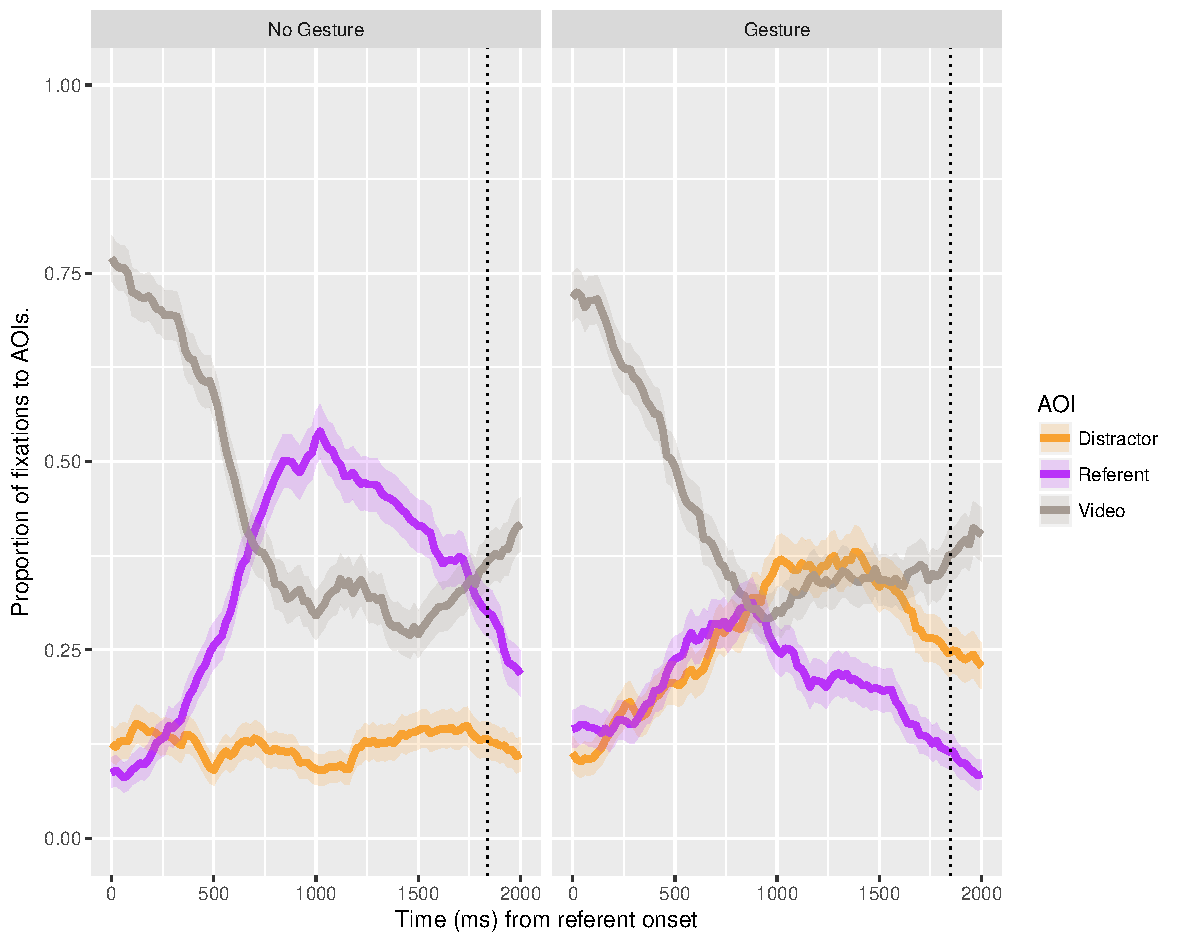
\includegraphics[width=\linewidth]{./img/e8_fixations.pdf}
  \caption{Eye-tracking results for Experiment 2: Proportion of fixations to each object (referent or distractor) and the video, from 0 to 2000 ms post-referent onset, calculated out of the total sum of fixations for each 20~ms time bin. Shaded areas represent $\pm$ 1 standard error of the mean.}
  \label{fig:v2_eye}
\end{figure}

\subsection{Mouse movements}
Figure \ref{fig:v2_mouse} shows the time-course of the proportions of cumulative distance the mouse moved towards the referent and distractor for 2000~ms from referent onset, split by presence of cue.
Analysis on the period from 0 to 800~ms post-referent onset patterned with the eye-tracking data:
Following no-cue videos, participants showed a tendency to move the mouse increasingly towards referent over this period (\resultsLM{1.90}{0.39}{=4.93}).
As with eye-movements, this referent-bias was greatly reduced following an adaptor gesture (\resultsLM{-2.46}{0.77}{=-3.19})

\begin{figure}[Ht]gesture
  \centering
	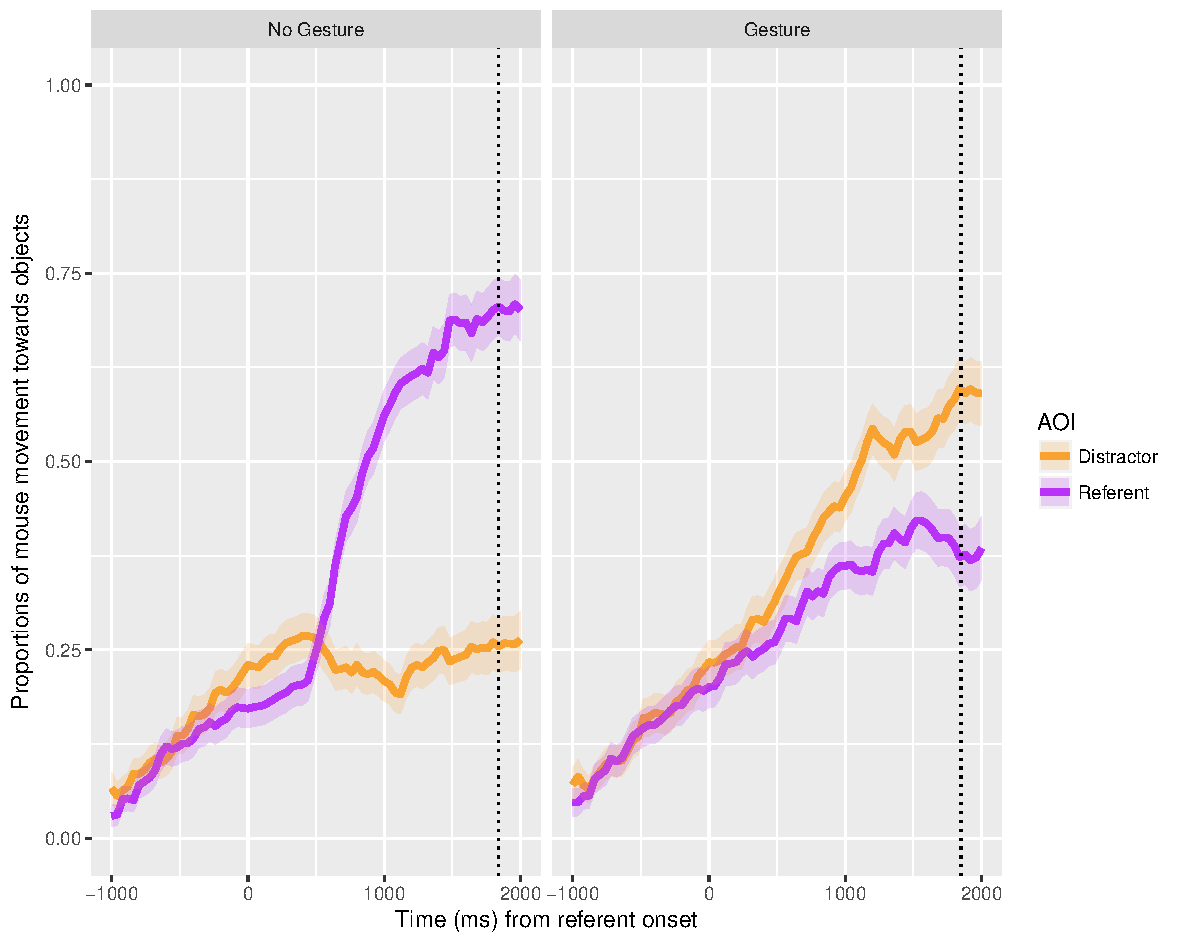
\includegraphics[width=\linewidth]{./img/e8_mouset.pdf}
  \caption{Mouse-tracking results for Experiment 2: Proportion of cumulative distance traveled toward each object from 0 to 2000 ms post-referent onset. Proportions were calculated from the total cumulative distance participants moved the mouse until that time bin (from speech-onset, when cursor was made visible). Shaded areas represent $\pm$ 1 standard error of the mean.}
  \label{fig:v2_mouse}
\end{figure}

\section{General discussion}
The studies presented here investigate the integration of visual information about a speaker into judgements of deception.
We manipulated the presentation of the speaker's non-verbal behaviours while measuring eye- and mouse- movements of the listener towards one of two possible final judgements about the veracity of an utterance.
In doing so, we explored the possibilities of whether listeners are relying upon a rule-of-thumb heuristic in associating visual cues to deception, or whether the link between gestures and perceived deception requires a more complex inferential process.
In the first experiment we studied a variety of both static and dynamic cues, and in Experiment 2 we focussed on the possibility that listeners link gestures to deception via inferencing about the speakers emotional state, specifically their level of anxiety during speech production.

In both experiments, listeners interpreted an increase in movement as a sign of dishonesty in the speaker.
This association is consistent with previous research on beliefs about and judgements on visual cues to deception, which shows that listeners perceive a range of nonverbal behaviours to indicate deceit \citep[e.g.][]{Zuckerman1981, Akehurst1996, Vrij2000}.
This result also parallels the finding in \citet{Loy2017} where disfluent (as opposed to fluent) utterances saw a bias to infer that the speaker was lying. 
The results from Experiment 1 additionally show that listeners' judgements of dishonesty were driven by both cues that were static (posture changes) and dynamic (body movements). 
Together, these findings suggest that listeners may have an implicit bias to judge a speaker as honest in the absence of any obvious potential cue to deception. 
More generally, they align with the `truth bias' commonly observed in deception literature, in which listeners have a tendency to judge a speaker as truthful, even when explicitly told the speaker may be dishonest \citep{Vrij2000}.

The time course of listeners' eye and mouse movements also showed the same pattern across both experiments:
Utterances presented with the speaker in a neutral posture and not gesturing biased listeners towards believing the speaker to be truthful, as shown by increased tendency to fixate on, move the mouse towards, and eventually click on the object which was named by the speaker. 
In contrast, utterances presented alongside a gesture cue (notably an adaptor) reduced this bias.
Importantly, this difference emerged during the initial stages of utterance processing, within 1170~ms post-referent onset in Experiment 1 and 800~ms post-onset in Experiment 2.
This suggests that listeners' early inferences about the veracity of an utterance were rapidly influenced by the speaker's body language.
Thus, we show that just like spoken manner of delivery, information presented in the visual channel can very quickly modulate a listeners' judgements about the speaker's intentions alongside processing of the lexical information. 

Interestingly, in both experiments, the bias towards the distractor --- signifying perceived dishonesty --- over the referent appeared approximately 1000~ms after the referent began, at a later point than previous versions of this paradigm in which speech disfluencies were found to modulate judgements of deception. 
This time course of events is difficult to reconcile with a view that listeners are relying on rule-of-thumb associations between visual cues and deception.

However, our results do not provide definitive evidence for a more complex two-step reasoning process associating adaptor gestures with deception via perceived nervousness: Although participants' judgements of deception were driven by the presence or absence of an adaptor, these judgements did not pattern with their ratings of how nervous the speaker appeared in each video beyond whether or not the video included a gesture.
%JK >> Jia, agreed, not sure if this is the best analysis really.
%ratings & judgements ARE linked, but this isn't very interesting (we chose gesture videos with high ratings, and no-gesture videos with low ratings). Looking at obj_clicked~rating on it's own doesn't tell us anything - is the correlation because of perceived nervousness or simply because of presence of gesture?.
%all I could think of was to sort of ask "are ratings correlated with object clicks beyond the presence of gesture?"
%but that Q really would have been answered better if we had a set of gestures which ranged in their ratings (to see if, e.g. a less nervous gesture would result in fewer deception judgements than a more-nervous gesture).

This suggests that the link between adaptors and perceived deception may not be a consequence of associating adaptors with anxiety and anxiety with deception.
Future research could investigate the possibility of other linking mechanisms, such as an inference via perception of the speaker's cognitive effort.

Our current results show that the integration of the visual channel in utterance processing can have a rapid and direct effect on a listener's pragmatic judgements, supporting the idea that communication is fundamentally multimodal: 
Speech and gesture interactively codetermine meaning.
However, the integration of visual cues to inform deception judgements appears to be more gradual than the integration of spoken cues.
To better understand how information in different modalities affect comprehension, further research would require investigating the effect of spoken delivery when the visual channel is also available --- for example, studying the time course of deception judgements when faced with one or both of a disfluency and an adaptor gesture.
%i.e. GVD 

\bibliography{./GCD}

\end{document}
